\section{Metodologia}

A metodologia será explanada de acordo com as etapas definidas na subseção \ref{subsec:etapas}.

\subsubsection*{Caracterização do problema e determinação do modelo}

Deseja-se avaliar a interação entre algumas variáveis de interesse e o tempo de queda de um ``helicóptero'' de papel. Para isso foi utilizado o modelo apresentado a na Figura \ref{fig:helicopter}, onde se pode ver os cortes e dobraduras a serem realizados. Pode-se notar que há diferentes dimensões que podem ser utilizadas no recorte, bem como a posição onde se pode colocar fita adesiva e um clipe de papel. As dimensões adotadas nesse \textbf{DoE} foram: 9,5 cm para comprimento do corpo (\emph{body length}) e comprimento das asas (\emph{wings length}) e 4 cm para a largura do corpo (\emph{body width}).

\begin{figure}[h]
  \centering
  \caption{Referência para criação dos modelos.}
  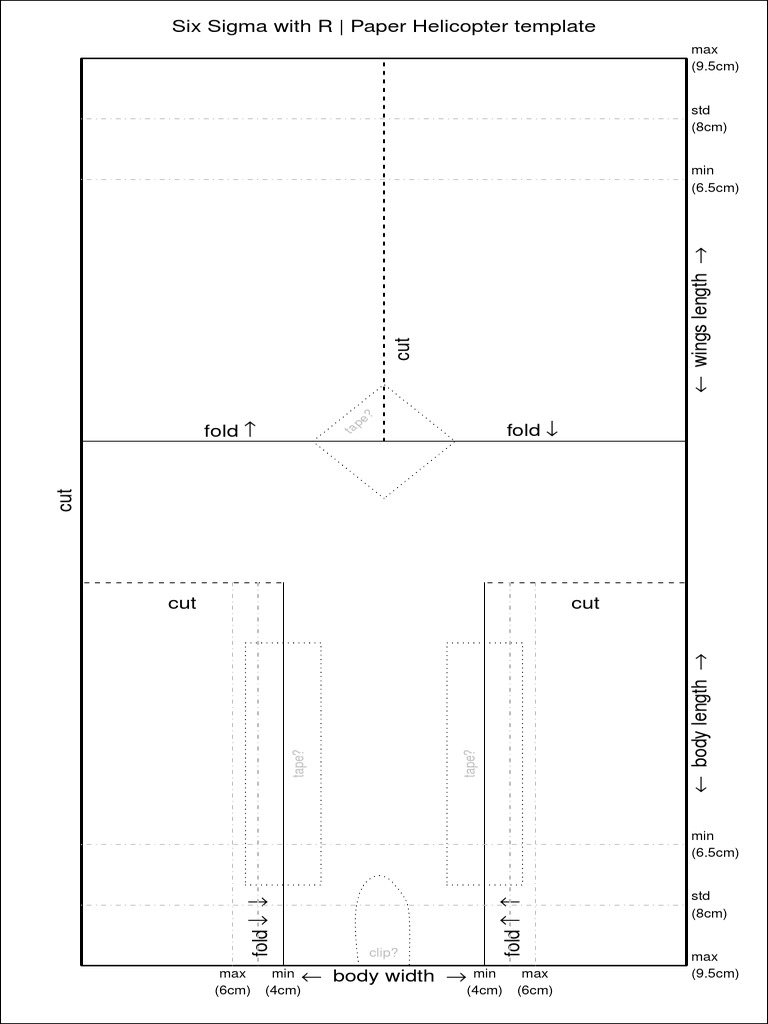
\includegraphics[scale=0.3]{images/helicopter.jpg}
  \label{fig:helicopter}
\end{figure}

Foram utilizadas folhas de papel A4 de gramatura 75 g/m$^2$ e clipe de papel n$^\circ$ 2/0, possuindo aproximadamente 1g. No modelo há três regiões destinadas a receber fita adesiva e para tanto foi utilizada fita adesiva transparente conforme a Figura \ref{fig:helimodel}. Além disso, a dobradura do corpo foi colada com uma camada fina de cola branca, de modo que a dobradura não abrisse durante o experimento.

\begin{figure}[h]
  \centering
  \caption{Referência para criação dos modelos.}
  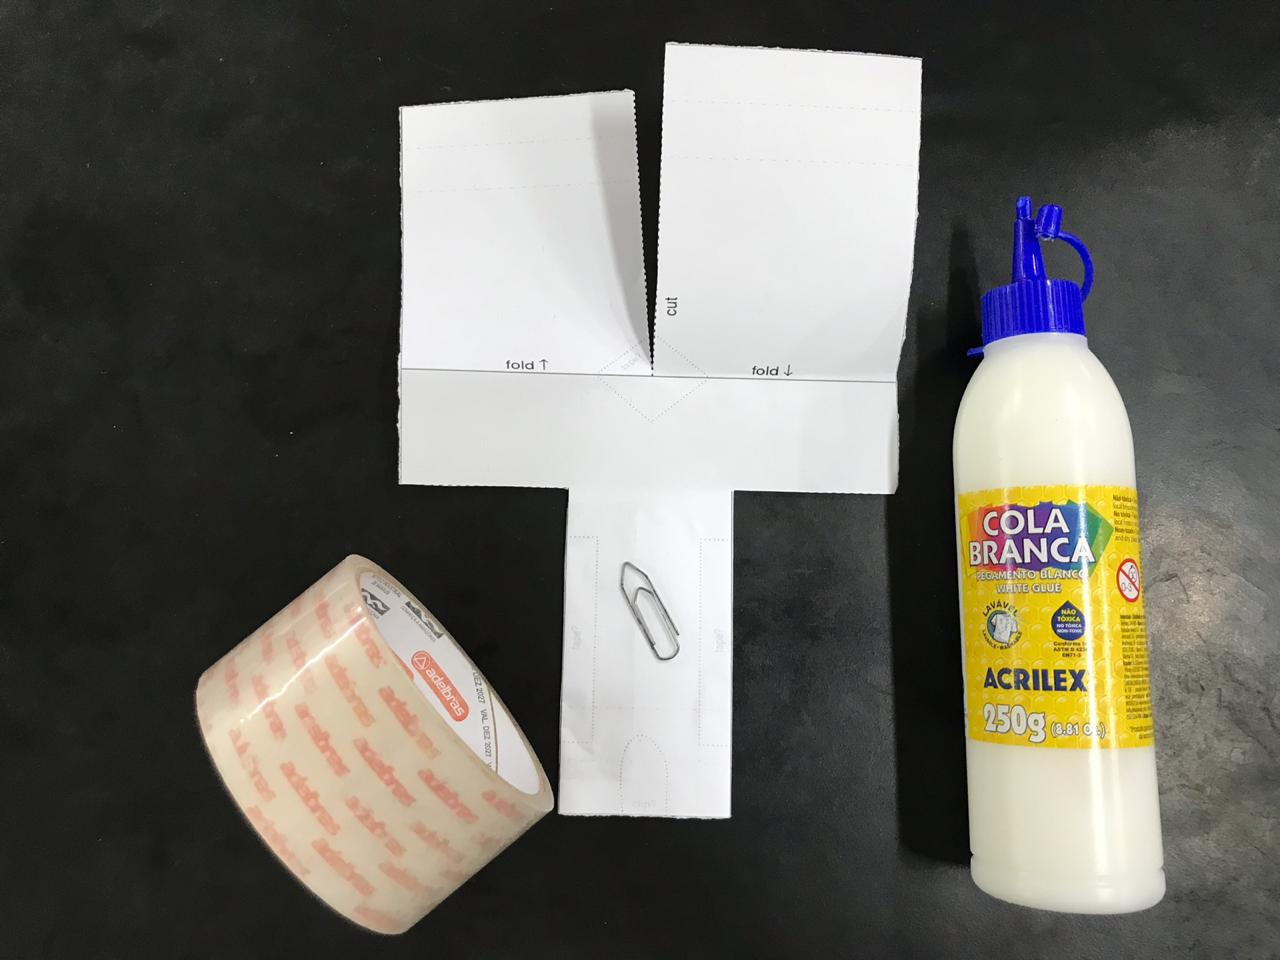
\includegraphics[scale=0.2]{images/helimodel.jpg}
  \label{fig:helimodel}
\end{figure}

\subsubsection*{Fatores de influência e variáveis de resposta}

Foram confeccionados 4 modelos básicos de ``helicópteros'', que sofreram alterações na massa por meio da adição de um clipe de papel na parte inferior, resultando em 8 modelos. Essas características podem ser resumidamente vistas na Tabela \ref{tab:carac}, onde foram selecionadas 4 variáveis independentes para o processo, cada uma dividida em dois níveis, e como variável dependente foi selecionado o tempo como parâmetro quantificador dos experimentos.

\begin{table}[h]
  \centering
  \caption{Características dos modelos.}
  % \resizebox{\linewidth}{!}{%
  \begin{tabular}{l|cc|c}
  \rowcolor[rgb]{0.784,0.784,0.784} \multicolumn{1}{c|}{\begin{tabular}[c]{@{}>{\cellcolor[rgb]{0.784,0.784,0.784}}c@{}}Variáveis\\independentes\end{tabular}} & \multicolumn{2}{c|}{Níveis } & \begin{tabular}[c]{@{}>{\cellcolor[rgb]{0.784,0.784,0.784}}c@{}}Variável\\dependente\end{tabular}  \\ 
  \hline
  Clipe                                                                                                                                                        & Com      & Sem               & \multirow{4}{*}{\begin{tabular}[c]{@{}c@{}}Tempo de\\queda\end{tabular}}                        \\
  Adesivo lateral                                                                                                                                              & Esquerda & Direita           &                                                                                                    \\
  Adesivo topo                                                                                                                                                 & Com      & Sem               &                                                                                                    \\
  Altura                                                                                                                                                       & 1,30 m   & 2,10 m            &                                                                                                   
  \end{tabular}
  \label{tab:carac}

  % }
  \end{table}

\subsubsection*{Determinação de planejamento do experimento}

A sequência de planejamento foi gerada aleatoriamente utilizando-se \emph{R}. Isso gerou um total de 16 experimentos, cada um deles realizado duas vezes, ou seja, duas medidas de tempo foram tomadas por duas pessoas diferentes utilizando cronômetros distintos. A partir disso, um tempo médio de queda foi estabelecido. A Tabela \ref{tab:plan} contempla o planejamento gerado em R. O valores ``S'' e ``C'' significam ``sem'' e ``com'', respectivamente; similarmente, ``E'' e ``D'' significam ``esquerda'' e ``direita''.

\begin{table}[ht]
  \caption{Ordenação do planejamento}
  \rowcolors{2}{gray!25}{white}
  \centering
  \begin{tabular}{lcccc}
    \rowcolor{gray!50}
    \hline
  Teste n$^\circ$ & Clipe & \multicolumn{1}{c}{\begin{tabular}[c]{@{}l@{}}Adesivo\\ topo\end{tabular}} & \multicolumn{1}{c}{\begin{tabular}[c]{@{}l@{}}Adesivo\\ lateral\end{tabular}}& Altura (m) \\ 
    \hline
  1 & S & S & E & 1.30 \\ 
    2 & C & S & E & 1.30 \\ 
    3 & S & C & E & 1.30 \\ 
    4 & C & C & E & 1.30 \\ 
    5 & S & S & D & 1.30 \\ 
    6 & C & S & D & 1.30 \\ 
    7 & S & C & D & 1.30 \\ 
    8 & C & C & D & 1.30 \\ 
    9 & S & S & E & 2.10 \\ 
    10 & C & S & E & 2.10 \\ 
    11 & S & C & E & 2.10 \\ 
    12 & C & C & E & 2.10 \\ 
    13 & S & S & D & 2.10 \\ 
    14 & C & S & D & 2.10 \\ 
    15 & S & C & D & 2.10 \\ 
    16 & C & C & D & 2.10 \\ 
     \hline
  \end{tabular}
  \label{tab:plan}
\end{table}

\subsubsection*{Condução do experimento}

O experimento foi realizado pelo mesma pessoa, no mesmo ambiente, sob mesmas condições climáticas, onde o helicóptero foi abandonado das alturas especificadas tendo sua base colocada nessas alturas, o que pode ser visto na Figura \ref{fig:amb}.

\subsubsection*{Análise dos dados e conclusões}

Uma análise de variância realizada utilizando \emph{R} gerou os dados que serão analisados na seção a seguir. Ela irá revelar o peso de cada variável dependente no tempo de queda, mostrando se é possível adotar um bom modelo linearizado para o fenômeno.

\newpage
\section*{}

\begin{figure}[t!]
  \caption{Ambiente de realização do experimento.}
  \begin{subfigure}{0.5\textwidth}
    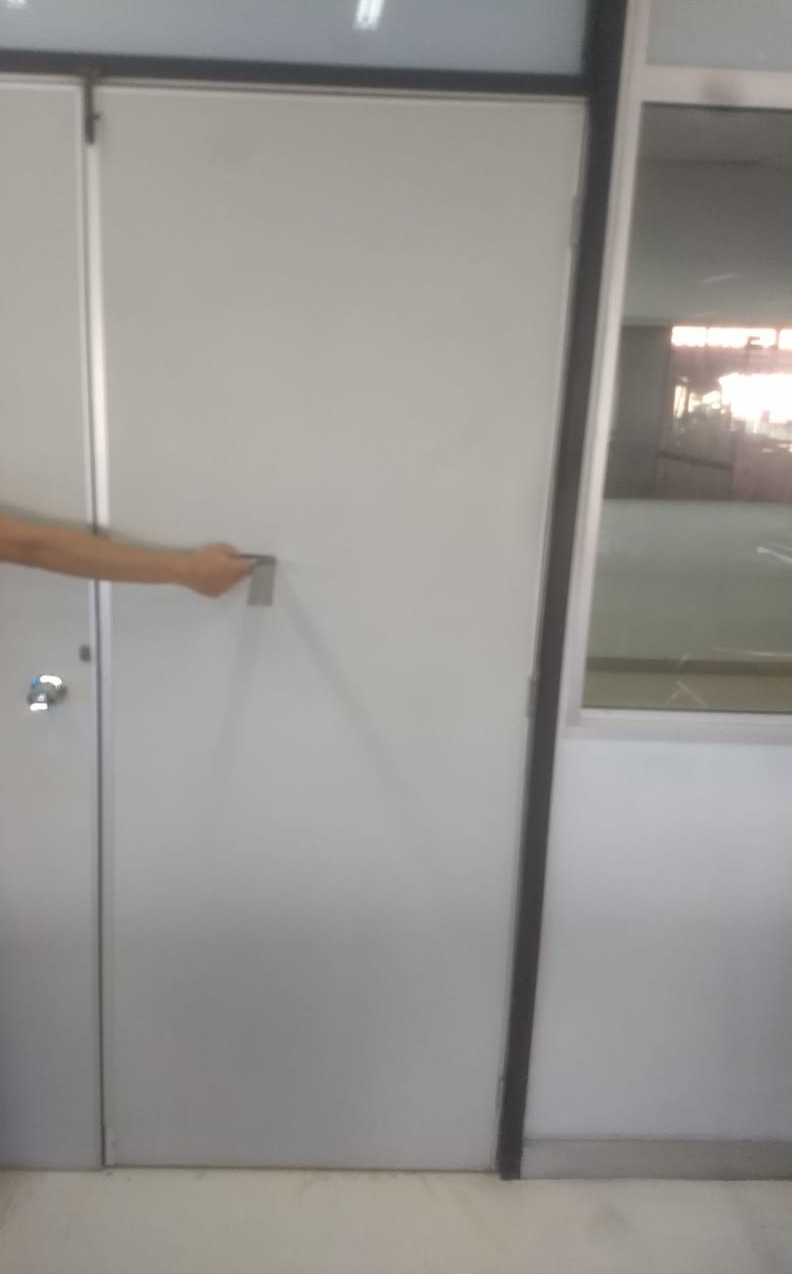
\includegraphics[width=0.9\linewidth]{images/altura130cm.jpg} 
    \caption{Altura de 1,30 m.}
  \end{subfigure}
  \begin{subfigure}{0.5\textwidth}
    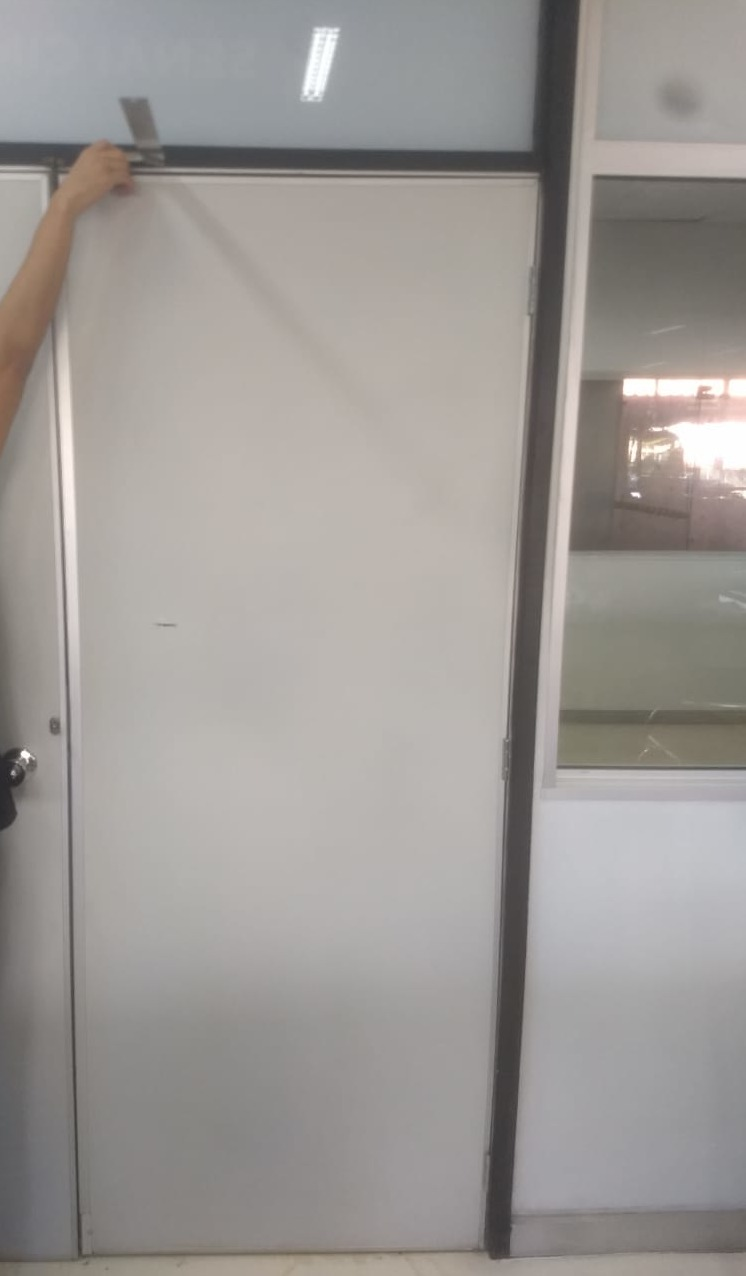
\includegraphics[width=0.9\linewidth, height = 10.75 cm]{images/altura210cm.jpg}
    \caption{Altura de 2,10 m.}
  \end{subfigure}
    \label{fig:amb}
\end{figure}